Given the theoretical and practical approaches studied previously, our own software development, which allows us to graphically display the relationships between criminal actors in the Criminal System of the Province of Chubut, is promoted as a vital support tool in decision-making criminal investigation of criminal gangs.
%Ante los enfoques teóricos y prácticos estudiados anteriormente, nuestro desarrollo de software propio, que permite mostrar de manera gráfica las relaciones entre actores delictuales en el Sistema Penal de la Provincia del Chubut, se potencia como una herramienta vital de apoyo en la toma de decisiones de la investigación penal de bandas delictivas.

Being able to visualize relationships between the people involved in criminal cases helps specialists to detect triangulations, transitivities and of course centralities in the Network. All this, added to the research evidence and the subject's own expertise complete an analysis tool to determine certain gangs or highly related groups.
%Poder visualizar relaciones entre las personas involucradas en casos penales ayuda a los especialistas a detectar triangulaciones, transitividades y por supuesto centralidades en la Red. Todo ello, sumado a los indicios de investigación y la propia expertís en la temática completan una herramienta de análisis para determinar ciertas bandas o grupos altamente relacionados.

In 2019, there were investigations linked to repeated thefts of LCD televisions at homes~\cite{noticiaLCDdiario}, as well as a series of consecutive events linked to the theft of safes in companies in the industrial park of the city of Trelew.
%En el año 2019 existieron investigaciones vinculadas a reiterados robos de televisores LCD en domicilios~\cite{noticiaLCDdiario}, como así también una serie de hechos consecutivos vinculados al robo de cajas fuertes en empresas del parque industrial de la ciudad de Trelew.

The UAC (Criminal Analysis Unit), an auxiliary agency of the Attorney General belonging to the Chubut Public Prosecutor's Office, served as a support team in the investigation of both modus operandi, making use of all the information from the tax files, general consultations and specific information contained in the Coirón System. The information referring to each person's \textit{groups of belonging} was of vital use, but it became an arduous job crossing information from people, to find the alleged criminal gangs behind these events.
%La UAC (Unidad de Análisis Criminal), organismo auxiliar de la Procuración General perteneciente al Ministerio Público Fiscal del Chubut, sirvió como equipo de apoyo en la investigación de ambos modus operandi, haciendo uso de toda la información de los legajos fiscales, consultas generales y específicas contenidas en el Sistema Coirón. Fue de vital uso la información referida a los \textit{grupos de pertenencia} de cada persona, pero devino en un arduo trabajo entrecruzando información de personas, para dar con las supuestas bandas delictivas detrás de estos hechos.

These investigations served as an initial kick to carry out this work and to be able to provide the information already contained in the criminal management system, in another way, in a more direct and visual way when investigating, which directly serves as support for decision-making. decisions in criminal gang investigations.
%Dichas investigaciones sirvieron como puntapié inicial para realizar este trabajo y poder facilitar la información ya contenida en el sistema de gestión penal, de otra manera, de una forma más directa y visual a la hora de investigar, que sirva directamente como apoyo a la toma de decisiones en las investigaciones de bandas delictivas. 

Below you can see a visualization extracted from this work, using as 
search filters two people (nodes 116587 and 145262) with many cases and relationships in the system, in order to find if there is any kind of direct relationship between them, and in turn. time if there are nodes that produce transitivities or are in turn central to other groups.
From the visualization, thanks to the link with the people identification office system, photographs were added to be placed in the nodes and make this work an even more powerful tool. Those people who have not been identified in court will not have a photograph. For legal reasons, the photographs have been blurred and identifiers have been placed instead of the real names of the people involved.
%A continuación se puede observar una visualización extraída de este trabajo, utilizando como filtros de búsqueda dos personas (nodos 116587 y 145262) con muchos casos y relaciones en el sistema, a fin de encontrar si existe algún tipo de relación directa entre ambos, y a su vez si existen nodos que produzcan transitividades o sean a su vez centrales de otros grupos.
%Desde la visualización se agregó gracias a la vinculación con el sistema de la oficina de identificación de personas, fotografías para colocar en los nodos y hacer de este trabajo una herramienta aún más potente. Aquellas personas que no hayan sido identificadas en sede judicial no tendrán fotografía. Por cuestiones judiciales se han desenfocado las fotografías y se han colocado identificadores en vez de los nombres reales de las personas intervinientes.
%\vspace{-10pt}
\begin{figure}
	\centering
	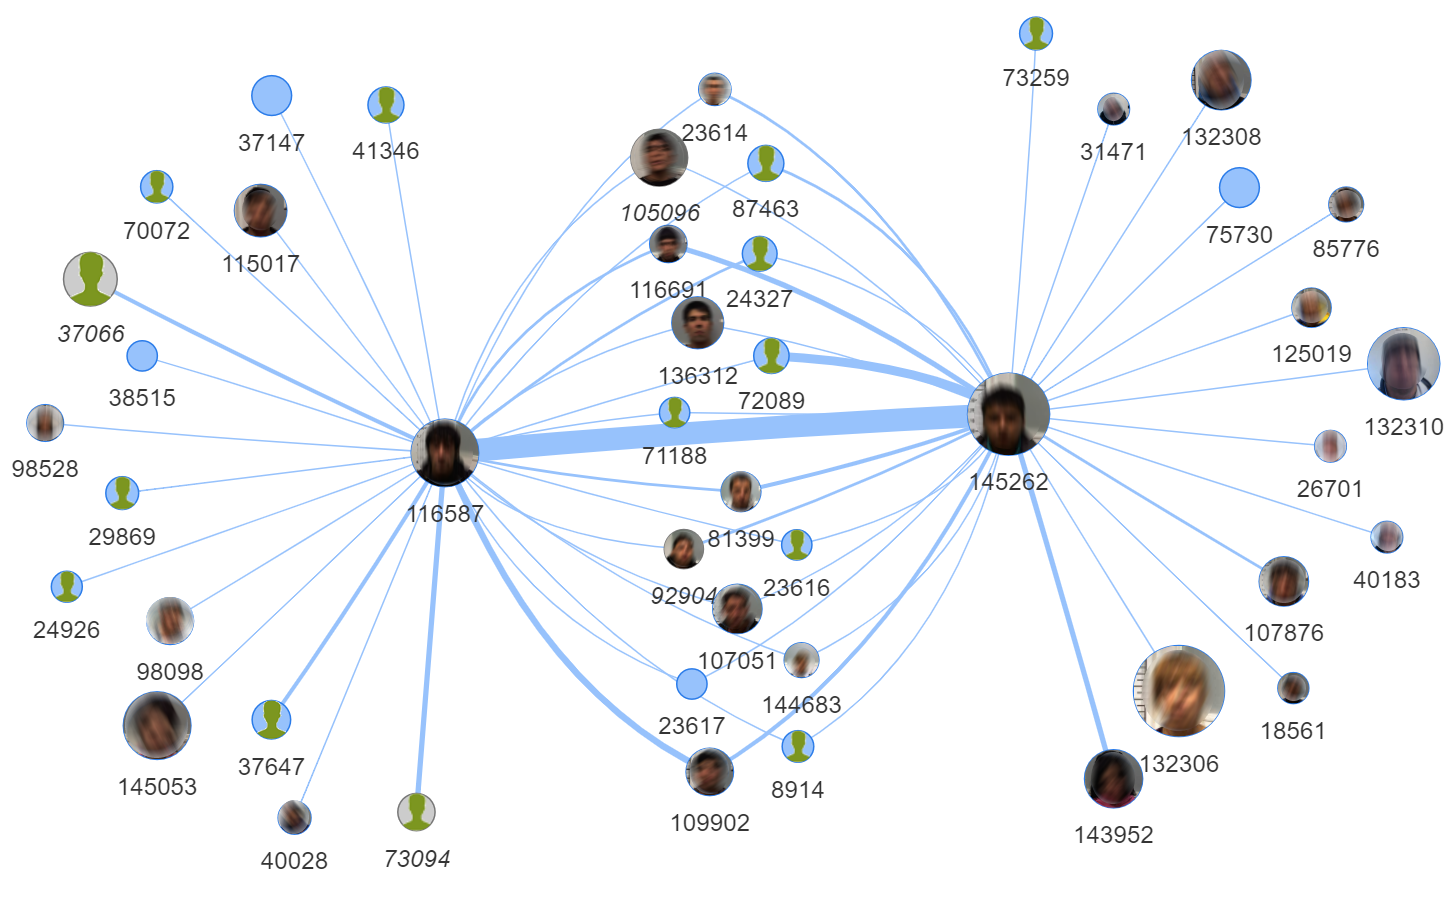
\includegraphics[width=0.75\linewidth]{hermanos-curruman.png}
	\caption{Relationship between two people. Photos are added.} 
	\label{fig:hermanos-curruman}
\end{figure}

%\vspace{-10pt}
As can be seen, in the central part of the image there are many people who are criminally related to both nodes in question. In this way, actions can be taken with respect to these people in order to find patterns of occurrence that link them to the possibility of identifying them as a supposed criminal gang.
%Como puede verse, existen en la parte central de la imagen muchas personas que se encuentran relacionadas delictualmente con ambos nodos en cuestión. De esta manera se pueden tomar acciones con respecto a estas personas en pos de encontrar patrones de ocurrencia que los vinculen ante la posibilidad de identificarlos como una supuesta banda delictiva. 